\documentclass[titlepage]{article}
\usepackage[T1]{fontenc}
\usepackage[utf8]{inputenc}
\usepackage{biblatex}
\usepackage{titling, lipsum}
\usepackage{graphicx}
\usepackage{indentfirst}
\usepackage{geometry}
\usepackage{hyperref} 
\usepackage{float}
\usepackage{enumitem}

\graphicspath{{./images/}}

\geometry{
 a4paper,
 total={170mm,257mm},
 margin=1in
}

\addbibresource{bibliography.bib}

\begin{document}
\begin{titlepage}
	{\centering
	{\scshape\huge Comparison of SLAM methods with CUDA implementation \par}
	\vspace{1cm}
	{\scshape\Large Course: Research project - GPU algorithms \par}}
	
	\vspace{1cm}
	\noindent\textbf{Coordinator}: Kaczmarski Krzysztof\\
	\textbf{Authors}: Rogala Michał, Stasiak Szymon, Śliwakowski Mateusz\\
	\textbf{Description}: This document covers three different SLAM methods with an emphasis on CUDA \mbox{implementation}\\
	\textbf{Code repository}: \href{https://github.com/Sliwson/cuda-slam}{https://github.com/Sliwson/cuda-slam}\\
	\textbf{Code license}: MIT\\
	\textbf{Input files}: Point clouds as .obj files\\

	\vfill
	{\large \today \par}
\end{titlepage}

\tableofcontents
\newpage

\section{Report goals}
%What we will know after reading this document?

The report is devoted to a research of SLAM methods using CUDA technology. We want to give a brief introduction what SLAM is and what are its applications. After reading the document you should know three different methods of approaching the problem, their advantages and disadvantages. The cornerstone of the work is answering the question - how well these methods can be converted to GPU architecture and how much will we gain?

\section{Problem statement}
%Description of the problem, motivating example, killer application, etc.

\subsection{Theoretical background}
\textbf{Simultaneous localization and mapping} (in short SLAM) is the computational problem of constructing or updating a map of an unknown environment while simultaneously keeping track of an agent's location within it \cite{ms-wiki1}. In theory the problem can be simplified to more mathematical definition - given two point sets $P_1 = \{x_1,\dots, x_n\}$ and $P_2=\{y_1, \dots, y_n\}$ find translation $t$ and rotation $R$ that minimizes the mean square error:
$$MSE(R, t) = \frac{1}{N}\sum_{i=1}{N}(x_i - Ry_i - t)^2$$

The reality, unfortunately, is much more complicated. Sizes of point sets might differ, clouds are unordered and noise points can occur.

\subsection{Applications}
The main field of SLAM application is robotics. There are a lot of machines that utilizes this algorithm to keep track of the space in which they are moving. The most popular are autonomous vacuum cleaners such as presented below.

\begin{figure}[H]
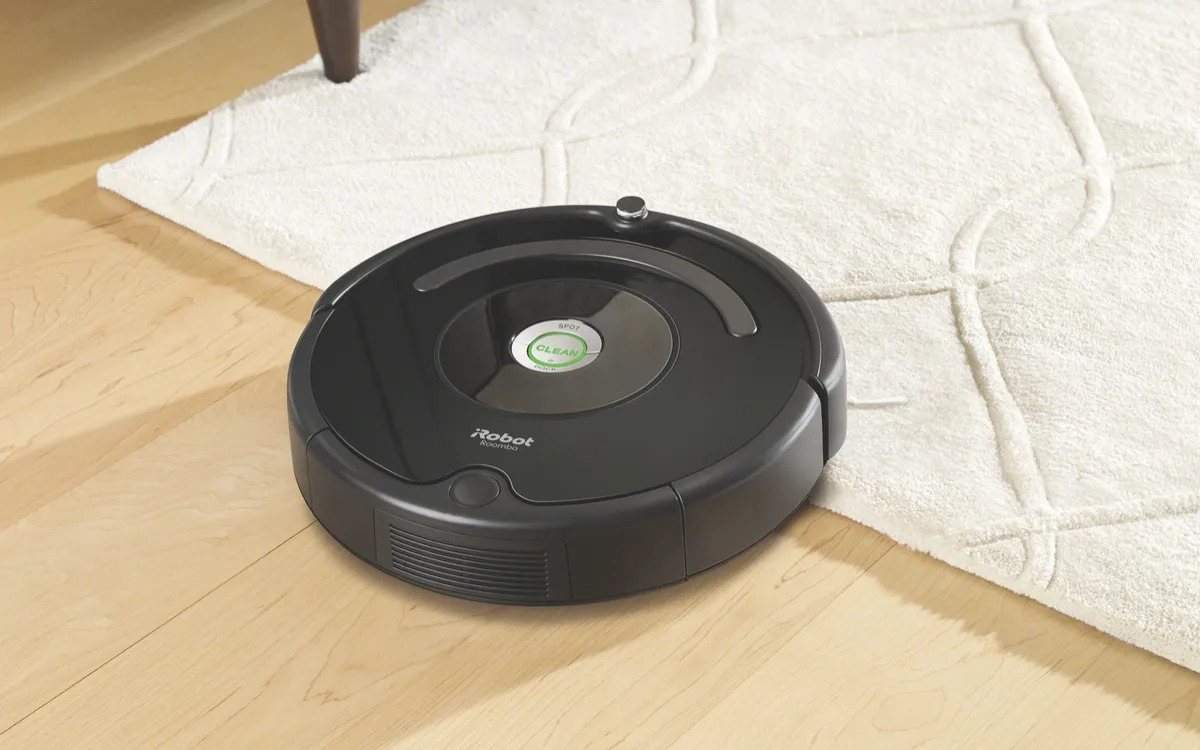
\includegraphics[width=\textwidth]{ms-img1.png}
\caption{Autonomous vacuum cleaner}
\end{figure}

Another popular application is mapping real life environments to digital equivalents. The programs produce \textit{Geospatial mappings} which can be later processed and analysed. Variety of different devices is used such as hand scanners, drone scanners or even satellites. Due to rapid technological progress nowadays, even smartphone cameras can be used to perform simple environmental scan.

\begin{figure}[H]
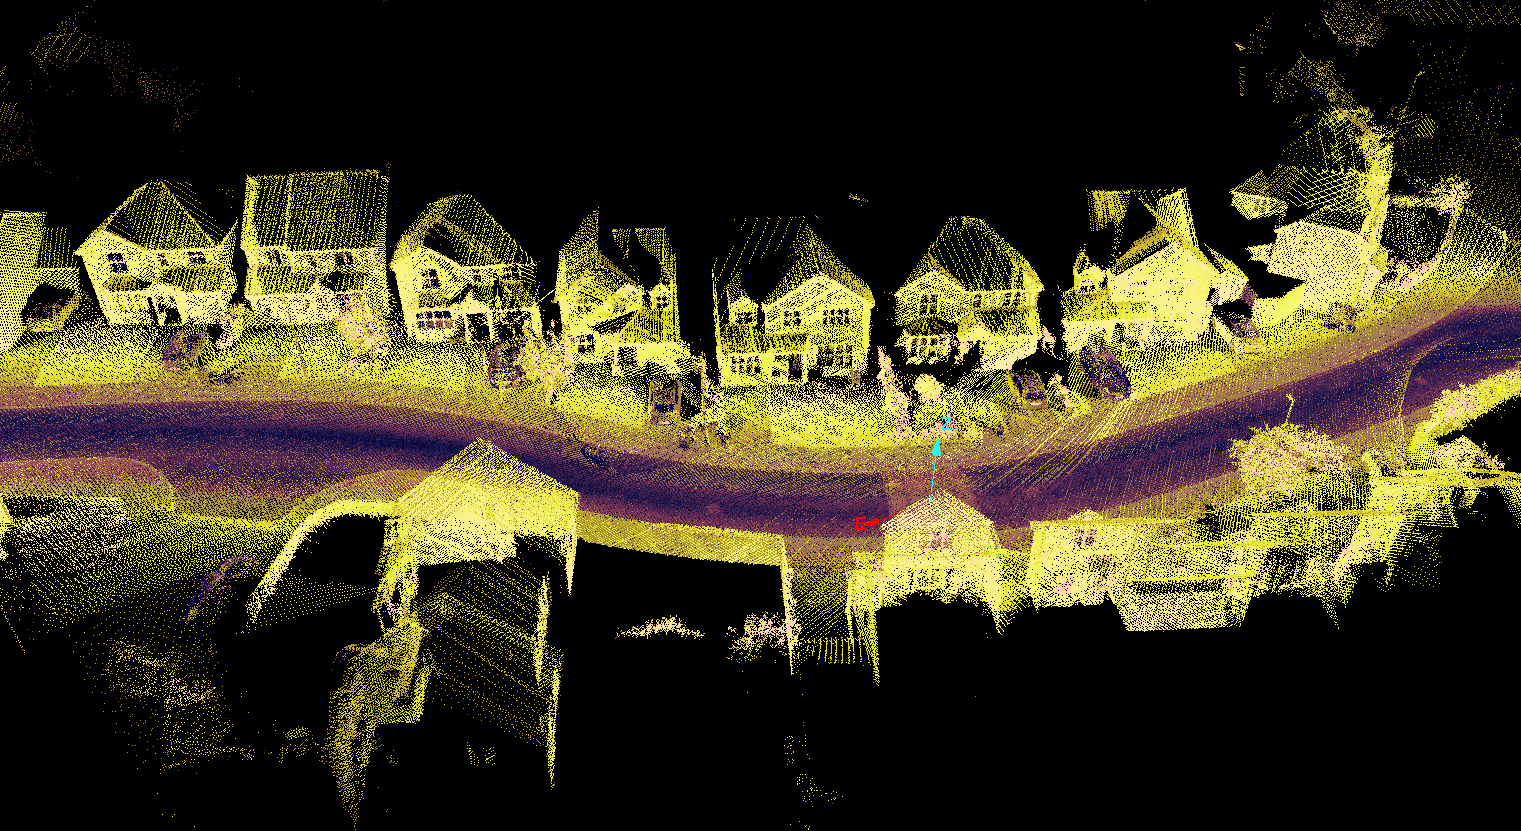
\includegraphics[width=\textwidth]{ms-img2.jpg}
\caption{3D laser scan}
\end{figure}

\section{Computational method}
%The most important ideas in the algorithm necessary to understand how it works.
%Are there any differences from other methods?
%Are there any novel ideas?

\subsection{Iterative Closest Point}
The most widely described and most popular method for solving SLAM problem is Iterative Closest Point algorithm. The main idea of the algorithm is stated below \cite{ms-pres1}:
\begin{enumerate}
\item Determine corresponding points.
\item Calculate translation and rotation using Singular Value Decomposition.
\item Apply calculated rotation and translation to the point cloud.
\item Compute Mean Squared Error.
\item If error decreased and it is greater than given threshold repeat all the steps.
\end{enumerate}

Various modifications have been proposed to this algorithm (such as sampling point sets, weighting the correspondences or rejecting outliers). However, in this project we focused on the base version of the method as it is good enough for comparison with the other algorithms.

\subsection{Noniterative Closest Point}

\subsection{Coherent Point Drift}

In this method alignment of two point sets is considered as a probability density estimation problem. One point set represents the Gaussian mixture model (GMM) centroinds. The second one represents the data points. Two point sets become aligned when optimum is reached. Method uses Expectation Maximization (EM) algorithm to find scale, rotation matrix and translation vector.\\
Main idea of coherent point drift can be presented in several steps:
\begin{itemize}[label={}]
\item E-step:
\begin{enumerate}
\item Compute probabilities matrix P. P describes probability of correspondence of points from both sets.
\end{enumerate}
\item M-step: 
\begin{enumerate}
\item Using P and point sets calculate matrix A.
\item Calculate rotation matrix using Singular Value Decomposition of matrix A.
\item Calculate scale and translation vector using point sets and SVD result.
\end{enumerate}
\item Repeat E-step and M-step until convergence.
\end{itemize}
Full algorithm was described by Andriy Myronenko and Xubo Song \cite{cpd}.\\
Algorithm has wide area available for improvements.\\
Firstly the size of P matrix is $N \times M$, where $N$ is size of first point set and $M$ is size of second point set. It requires a lot of memory to keep matrix of this size, so instead we can calculate vectors: $P1$, $P^T 1$ and matrix $PX$, where $1$ is vector of all ones and $X$ is first point set. Using these vectors and matrix we can achieve the same result even faster because in calculations we had to multiply P matrix with ones vector and we have already done it.\\
Secondly the main bottleneck of algorithm is the calculation of matrix-vector products $P1$, $P^T1$ and $PX$. This is done with $O(MN)$ complexity. The fast Gauss transform, introduced by Greengard and Strain \cite{fgt}, reduces complexity to only $O(M+N)$.
\section{Program architecture}
%Short description on the modules of the system, requirements, dependencies, etc.
\subsection{Project structure}
The solution consists of three projects:
\begin{itemize}
\item \textit{common} - static library project, contains all elements that are shared between cpu and gpu implementations.
\item \textit{cpu-slam} - executable project, contains implementation of slam methods for cpu and cpu main.
\item \textit{gpu-slam} - executable project, contains implementaion of slam methods for gpu and gpu main.
\end{itemize}

\section{Program architecture}
%Short description on the modules of the system, requirements, dependencies, etc.
\subsection{Project structure}
The solution consists of three projects:
\begin{itemize}
\item \textit{common} - static library project, contains all elements that are shared between cpu and gpu implementations.
\item \textit{cpu-slam} - executable project, contains implementation of slam methods for cpu and cpu main.
\item \textit{gpu-slam} - executable project, contains implementaion of slam methods for gpu and gpu main.
\end{itemize}

\subsection{Modules}
The project is constructed using several modules:
\begin{itemize}
\item \textit{Renderer} - implemented in \textit{common} project. Capable of rendering point clouds in different colors. Can be used multiple times in one executable launch. Widely using for results visualisation.
\item \textit{CloudLoader} - implemented in \textit{common} project. Module responsible for loading .obj point clouds.
\item \textit{Configuration} - implemented in \textit{common} project. Module representing configuration, tightly coupled with \textit{ConfigParser} which allows loading configuration from .json files.
\item \textit{TestRunner} - implemented in \textit{common} project. Module used to define and run benchmarks.
\item \textit{Algorithms} - implemented in \textit{cuda-slam} as well as \textit{cpu-slam}. Each algorithm is implemented in separate file as a global function in appropriate namespace. Some operations that are common for cpu as well as gpu are implemented in \textit{common} project.
\end{itemize}

\subsection{Dependencies}
\begin{itemize}
\item \textit{Assimp} - for cloud loading.
\item \textit{Eigen} - for cpu matrix operations.
\item \textit{Glad} - wrapper for OpenGL.
\item \textit{GLFW} - for window system.
\item \textit{Nlohmann/json} - for configuration parsing.
\item \textit{CuBLAS} - for gpu matrix operations.
\end{itemize}

\section{Input data description}
%File formats, api used to read, dependencies, data sources, etc.
%Is there any institution providing the input data?
%References to public databases.

As we wanted to keep the input simple we decided to use .obj files as the point clouds. It is easy to find multiple different models in this format which allowed us to test the algorithms on multiple distinctive samples. Furthermore, one can edit .obj files using for example \textit{Blender} to add noise or even cut off part of the cloud. We found that method most convenient to simulate real life conditions as 3D scanners data has to be processed using methods that are beyond the scope of our work.

\begin{figure}[H]
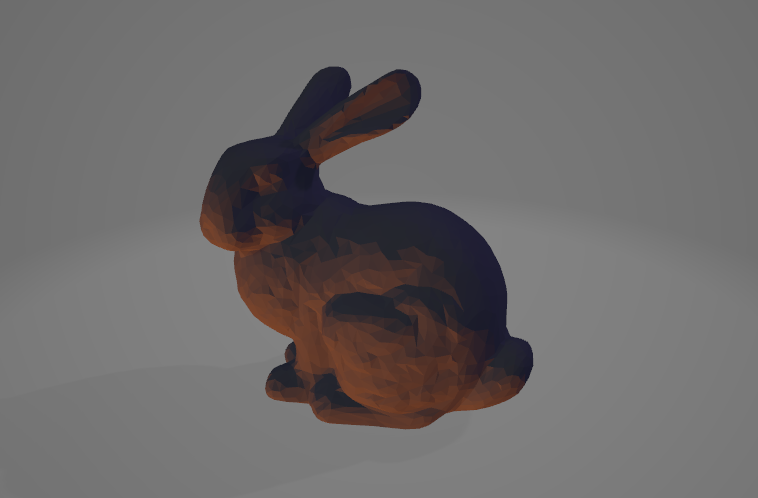
\includegraphics[width=\textwidth]{ms-bunny.png}
\caption{Sample .obj file}
\end{figure}

\section{Execution, configuration and user guide}
How can one replicate the experiments?
Any relevant information and runtime howtos.

\section{Description of the results}
%Performance of the system for different input data/parameters.
%How we understand the results and why are they correct?
%Can we formulate any conclusions from the experiments?

\subsection{Speed}

\subsection{Stability}

\subsection{Noise and outliers tolerance}

\subsection{Convergence ranges}

\section{Remarks}
Any remarks to the results and methods.

\section{Future works}
%What do we want to do in future, improvements.

\subsection{Iterative Closest Point}
We implemented a solid ground base for development of ICP algorithm. There are a lot of ways it can be improved but the most important would be enhancing performance of correspondences step as it is critical for the whole method execution time.

\subsection{Coherent Point Drift}
We implemented whole rigid part of the algorithm on cpu, including FGT. Unfortunately FGT was not implemented on GPU due to complexity of this solution and lack of reliable external implementation. This is main area of improvement for GPU solution. Coherent Point Drift also has affine and non-rigid versions that are worth mentioning. Future works can mainly focus on improving GPU solution and moving to non-rigid transformations.


\subsection{Common improvements}
The key to performant SLAM for big clouds is sampling. We have not covered it in our work as it is a broad topic and mostly dependent of the specific application of the algorithm. Although, there is no contraindication to use sampled clouds as the input of our program so everybody can make their own experiments in that field.

\newpage
\printbibliography

\end{document}

